\scanpage{167}
Validité des théorèmes de dualité

1) \uline{Dualité globale}
\[
\operatorname{Hom}(F_\bullet,\mathbb{R}^{!}f(G^{\bullet}))\xleftarrow{\sim}\operatorname{Hom}(\mathbb{R}_{!}f(F_\bullet),G^{\bullet})
\]
$f:(X,A_X)\unsure{\text{---}|\longrightarrow}(Y,A_Y)$ morphisme \uline{compactifiable} et \uline{\unsure{lissifiable}} de préschémas, annelés par $A_X$ et $A_Y$, \deleted{\unsure{des}} faisceaux d'anneaux \deleted{de \uline{torsion}} tels que pour tt pt géom. $\bar{y}$ de $Y$, $\exists n_{\bar{y}}\geq1$ \unsure{que} $n_{\bar{y}}A_{Y,\bar{y}}=\deleted{\text{est un anneau}}0$ $n_{\bar{y}}$ premier à $\operatorname{car}k(\bar{y})$.

2) \uline{Dualité locale}
\[
F_\bullet\simeq\unsure{\underline{D}|D}_X\unsure{\underline{D}|D}_X(F_\bullet)\quad\text{isom,}\quad\unsure{\underline{D}|D}_X(F_\bullet)\text{ à ch. constructible,}
\]
$X$ préschéma \deleted{\unsure{loc.}} noeth. \uline{régulier} annelé par $A_X$ faisceau d'anneaux loc. ct à fibres \deleted{\unsure{noethériennes}} \unsure{qui sont} des anneaux de torsion noethériens, premiers aux car. résiduelles

$R_X^{\bullet}$ un \inserted{complexe de} faisceaux de $A_X$-Modules loc. const., et dualisant \inserted{sur les} fibres \deleted{géométriques}
\[
\unsure{\underline{D}|D}_X(F_\bullet)=\unsure{\mathrm{R}|\mathbb{R}}\mathcal{H}om(F_\bullet,\unsure{A_X|R_X})
\]
\[
F_\bullet\in\operatorname{Ob}D^b(X)
\]
\margin{\figure{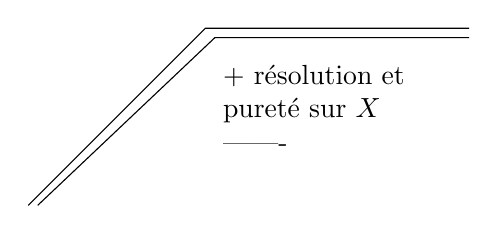
\begin{tikzpicture}[x=1cm,y=1cm]
\draw (0,0)--(2.25,2.25)--(5.6,2.25);
\draw (.12,0)--(2.37,2.13)--(5.6,2.13);
\node[anchor=north west,align=left] at (2.35,1.9) {+ résolution et\\pureté sur $X$\\-------};
\end{tikzpicture}}}
\margin{166}
